\section{Poprawność sterowania i punkt pracy stanowiska}
\label{lab:zad1}

Przeprowadzono symulację odpowiedzi procesu dla punktu pracy. 
Ustalone zostały stałe sygnały sterujące G1 = \num{32} i  Z = \num{0} .

\begin{figure}[H] 
    \centering
    % This file was created by matlab2tikz.
%
\definecolor{mycolor1}{rgb}{0.00000,0.44700,0.74100}%
%
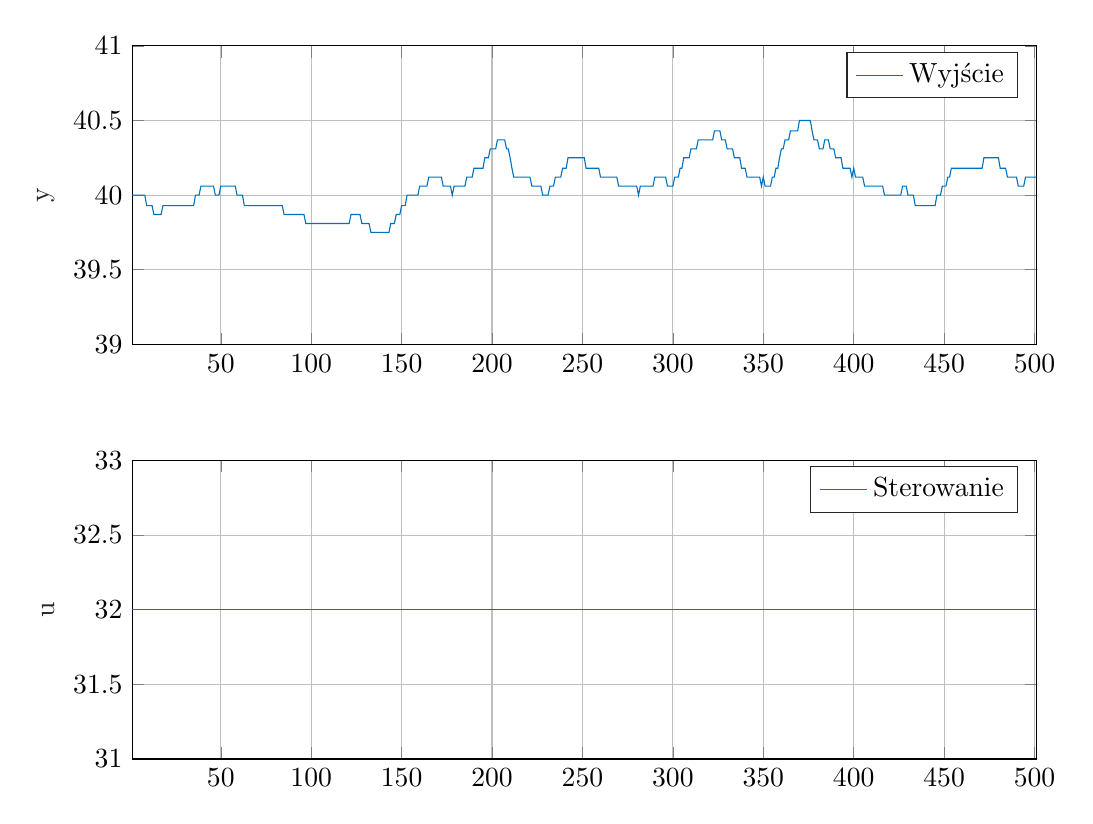
\begin{tikzpicture}

\begin{axis}[%
width=4.521in,
height=1.493in,
at={(0.758in,2.554in)},
scale only axis,
xmin=1,
xmax=501,
ymin=39,
ymax=41,
ylabel style={font=\color{white!15!black}},
ylabel={y},
axis background/.style={fill=white},
xmajorgrids,
ymajorgrids,
legend style={legend cell align=left, align=left, draw=white!15!black}
]
\addplot [color=mycolor1]
  table[row sep=crcr]{%
1	40\\
2	40\\
3	40\\
4	40\\
5	40\\
6	40\\
7	40\\
8	40\\
9	39.93\\
10	39.93\\
11	39.93\\
12	39.93\\
13	39.87\\
14	39.87\\
15	39.87\\
16	39.87\\
17	39.87\\
18	39.93\\
19	39.93\\
20	39.93\\
21	39.93\\
22	39.93\\
23	39.93\\
24	39.93\\
25	39.93\\
26	39.93\\
27	39.93\\
28	39.93\\
29	39.93\\
30	39.93\\
31	39.93\\
32	39.93\\
33	39.93\\
34	39.93\\
35	39.93\\
36	40\\
37	40\\
38	40\\
39	40.06\\
40	40.06\\
41	40.06\\
42	40.06\\
43	40.06\\
44	40.06\\
45	40.06\\
46	40.06\\
47	40\\
48	40\\
49	40\\
50	40.06\\
51	40.06\\
52	40.06\\
53	40.06\\
54	40.06\\
55	40.06\\
56	40.06\\
57	40.06\\
58	40.06\\
59	40\\
60	40\\
61	40\\
62	40\\
63	39.93\\
64	39.93\\
65	39.93\\
66	39.93\\
67	39.93\\
68	39.93\\
69	39.93\\
70	39.93\\
71	39.93\\
72	39.93\\
73	39.93\\
74	39.93\\
75	39.93\\
76	39.93\\
77	39.93\\
78	39.93\\
79	39.93\\
80	39.93\\
81	39.93\\
82	39.93\\
83	39.93\\
84	39.93\\
85	39.87\\
86	39.87\\
87	39.87\\
88	39.87\\
89	39.87\\
90	39.87\\
91	39.87\\
92	39.87\\
93	39.87\\
94	39.87\\
95	39.87\\
96	39.87\\
97	39.81\\
98	39.81\\
99	39.81\\
100	39.81\\
101	39.81\\
102	39.81\\
103	39.81\\
104	39.81\\
105	39.81\\
106	39.81\\
107	39.81\\
108	39.81\\
109	39.81\\
110	39.81\\
111	39.81\\
112	39.81\\
113	39.81\\
114	39.81\\
115	39.81\\
116	39.81\\
117	39.81\\
118	39.81\\
119	39.81\\
120	39.81\\
121	39.81\\
122	39.87\\
123	39.87\\
124	39.87\\
125	39.87\\
126	39.87\\
127	39.87\\
128	39.81\\
129	39.81\\
130	39.81\\
131	39.81\\
132	39.81\\
133	39.75\\
134	39.75\\
135	39.75\\
136	39.75\\
137	39.75\\
138	39.75\\
139	39.75\\
140	39.75\\
141	39.75\\
142	39.75\\
143	39.75\\
144	39.81\\
145	39.81\\
146	39.81\\
147	39.87\\
148	39.87\\
149	39.87\\
150	39.93\\
151	39.93\\
152	39.93\\
153	40\\
154	40\\
155	40\\
156	40\\
157	40\\
158	40\\
159	40\\
160	40.06\\
161	40.06\\
162	40.06\\
163	40.06\\
164	40.06\\
165	40.12\\
166	40.12\\
167	40.12\\
168	40.12\\
169	40.12\\
170	40.12\\
171	40.12\\
172	40.12\\
173	40.06\\
174	40.06\\
175	40.06\\
176	40.06\\
177	40.06\\
178	40\\
179	40.06\\
180	40.06\\
181	40.06\\
182	40.06\\
183	40.06\\
184	40.06\\
185	40.06\\
186	40.12\\
187	40.12\\
188	40.12\\
189	40.12\\
190	40.18\\
191	40.18\\
192	40.18\\
193	40.18\\
194	40.18\\
195	40.18\\
196	40.25\\
197	40.25\\
198	40.25\\
199	40.31\\
200	40.31\\
201	40.31\\
202	40.31\\
203	40.37\\
204	40.37\\
205	40.37\\
206	40.37\\
207	40.37\\
208	40.31\\
209	40.31\\
210	40.25\\
211	40.18\\
212	40.12\\
213	40.12\\
214	40.12\\
215	40.12\\
216	40.12\\
217	40.12\\
218	40.12\\
219	40.12\\
220	40.12\\
221	40.12\\
222	40.06\\
223	40.06\\
224	40.06\\
225	40.06\\
226	40.06\\
227	40.06\\
228	40\\
229	40\\
230	40\\
231	40\\
232	40.06\\
233	40.06\\
234	40.06\\
235	40.12\\
236	40.12\\
237	40.12\\
238	40.12\\
239	40.18\\
240	40.18\\
241	40.18\\
242	40.25\\
243	40.25\\
244	40.25\\
245	40.25\\
246	40.25\\
247	40.25\\
248	40.25\\
249	40.25\\
250	40.25\\
251	40.25\\
252	40.18\\
253	40.18\\
254	40.18\\
255	40.18\\
256	40.18\\
257	40.18\\
258	40.18\\
259	40.18\\
260	40.12\\
261	40.12\\
262	40.12\\
263	40.12\\
264	40.12\\
265	40.12\\
266	40.12\\
267	40.12\\
268	40.12\\
269	40.12\\
270	40.06\\
271	40.06\\
272	40.06\\
273	40.06\\
274	40.06\\
275	40.06\\
276	40.06\\
277	40.06\\
278	40.06\\
279	40.06\\
280	40.06\\
281	40\\
282	40.06\\
283	40.06\\
284	40.06\\
285	40.06\\
286	40.06\\
287	40.06\\
288	40.06\\
289	40.06\\
290	40.12\\
291	40.12\\
292	40.12\\
293	40.12\\
294	40.12\\
295	40.12\\
296	40.12\\
297	40.06\\
298	40.06\\
299	40.06\\
300	40.06\\
301	40.12\\
302	40.12\\
303	40.12\\
304	40.18\\
305	40.18\\
306	40.25\\
307	40.25\\
308	40.25\\
309	40.25\\
310	40.31\\
311	40.31\\
312	40.31\\
313	40.31\\
314	40.37\\
315	40.37\\
316	40.37\\
317	40.37\\
318	40.37\\
319	40.37\\
320	40.37\\
321	40.37\\
322	40.37\\
323	40.43\\
324	40.43\\
325	40.43\\
326	40.43\\
327	40.37\\
328	40.37\\
329	40.37\\
330	40.31\\
331	40.31\\
332	40.31\\
333	40.31\\
334	40.25\\
335	40.25\\
336	40.25\\
337	40.25\\
338	40.18\\
339	40.18\\
340	40.18\\
341	40.12\\
342	40.12\\
343	40.12\\
344	40.12\\
345	40.12\\
346	40.12\\
347	40.12\\
348	40.12\\
349	40.06\\
350	40.12\\
351	40.06\\
352	40.06\\
353	40.06\\
354	40.06\\
355	40.12\\
356	40.12\\
357	40.18\\
358	40.18\\
359	40.25\\
360	40.31\\
361	40.31\\
362	40.37\\
363	40.37\\
364	40.37\\
365	40.43\\
366	40.43\\
367	40.43\\
368	40.43\\
369	40.43\\
370	40.5\\
371	40.5\\
372	40.5\\
373	40.5\\
374	40.5\\
375	40.5\\
376	40.5\\
377	40.43\\
378	40.37\\
379	40.37\\
380	40.37\\
381	40.31\\
382	40.31\\
383	40.31\\
384	40.37\\
385	40.37\\
386	40.37\\
387	40.31\\
388	40.31\\
389	40.31\\
390	40.25\\
391	40.25\\
392	40.25\\
393	40.25\\
394	40.18\\
395	40.18\\
396	40.18\\
397	40.18\\
398	40.18\\
399	40.12\\
400	40.18\\
401	40.12\\
402	40.12\\
403	40.12\\
404	40.12\\
405	40.12\\
406	40.06\\
407	40.06\\
408	40.06\\
409	40.06\\
410	40.06\\
411	40.06\\
412	40.06\\
413	40.06\\
414	40.06\\
415	40.06\\
416	40.06\\
417	40\\
418	40\\
419	40\\
420	40\\
421	40\\
422	40\\
423	40\\
424	40\\
425	40\\
426	40\\
427	40.06\\
428	40.06\\
429	40.06\\
430	40\\
431	40\\
432	40\\
433	40\\
434	39.93\\
435	39.93\\
436	39.93\\
437	39.93\\
438	39.93\\
439	39.93\\
440	39.93\\
441	39.93\\
442	39.93\\
443	39.93\\
444	39.93\\
445	39.93\\
446	40\\
447	40\\
448	40\\
449	40.06\\
450	40.06\\
451	40.06\\
452	40.12\\
453	40.12\\
454	40.18\\
455	40.18\\
456	40.18\\
457	40.18\\
458	40.18\\
459	40.18\\
460	40.18\\
461	40.18\\
462	40.18\\
463	40.18\\
464	40.18\\
465	40.18\\
466	40.18\\
467	40.18\\
468	40.18\\
469	40.18\\
470	40.18\\
471	40.18\\
472	40.25\\
473	40.25\\
474	40.25\\
475	40.25\\
476	40.25\\
477	40.25\\
478	40.25\\
479	40.25\\
480	40.25\\
481	40.18\\
482	40.18\\
483	40.18\\
484	40.18\\
485	40.12\\
486	40.12\\
487	40.12\\
488	40.12\\
489	40.12\\
490	40.12\\
491	40.06\\
492	40.06\\
493	40.06\\
494	40.06\\
495	40.12\\
496	40.12\\
497	40.12\\
498	40.12\\
499	40.12\\
500	40.12\\
501	40.12\\
};
\addlegendentry{Wyjście}

\end{axis}

\begin{axis}[%
width=4.521in,
height=1.493in,
at={(0.758in,0.481in)},
scale only axis,
xmin=1,
xmax=501,
ymin=31,
ymax=33,
ylabel style={font=\color{white!15!black}},
ylabel={u},
axis background/.style={fill=white},
xmajorgrids,
ymajorgrids,
legend style={legend cell align=left, align=left, draw=white!15!black}
]
\addplot[const plot, color=mycolor1] table[row sep=crcr] {%
1	32\\
2	32\\
3	32\\
4	32\\
5	32\\
6	32\\
7	32\\
8	32\\
9	32\\
10	32\\
11	32\\
12	32\\
13	32\\
14	32\\
15	32\\
16	32\\
17	32\\
18	32\\
19	32\\
20	32\\
21	32\\
22	32\\
23	32\\
24	32\\
25	32\\
26	32\\
27	32\\
28	32\\
29	32\\
30	32\\
31	32\\
32	32\\
33	32\\
34	32\\
35	32\\
36	32\\
37	32\\
38	32\\
39	32\\
40	32\\
41	32\\
42	32\\
43	32\\
44	32\\
45	32\\
46	32\\
47	32\\
48	32\\
49	32\\
50	32\\
51	32\\
52	32\\
53	32\\
54	32\\
55	32\\
56	32\\
57	32\\
58	32\\
59	32\\
60	32\\
61	32\\
62	32\\
63	32\\
64	32\\
65	32\\
66	32\\
67	32\\
68	32\\
69	32\\
70	32\\
71	32\\
72	32\\
73	32\\
74	32\\
75	32\\
76	32\\
77	32\\
78	32\\
79	32\\
80	32\\
81	32\\
82	32\\
83	32\\
84	32\\
85	32\\
86	32\\
87	32\\
88	32\\
89	32\\
90	32\\
91	32\\
92	32\\
93	32\\
94	32\\
95	32\\
96	32\\
97	32\\
98	32\\
99	32\\
100	32\\
101	32\\
102	32\\
103	32\\
104	32\\
105	32\\
106	32\\
107	32\\
108	32\\
109	32\\
110	32\\
111	32\\
112	32\\
113	32\\
114	32\\
115	32\\
116	32\\
117	32\\
118	32\\
119	32\\
120	32\\
121	32\\
122	32\\
123	32\\
124	32\\
125	32\\
126	32\\
127	32\\
128	32\\
129	32\\
130	32\\
131	32\\
132	32\\
133	32\\
134	32\\
135	32\\
136	32\\
137	32\\
138	32\\
139	32\\
140	32\\
141	32\\
142	32\\
143	32\\
144	32\\
145	32\\
146	32\\
147	32\\
148	32\\
149	32\\
150	32\\
151	32\\
152	32\\
153	32\\
154	32\\
155	32\\
156	32\\
157	32\\
158	32\\
159	32\\
160	32\\
161	32\\
162	32\\
163	32\\
164	32\\
165	32\\
166	32\\
167	32\\
168	32\\
169	32\\
170	32\\
171	32\\
172	32\\
173	32\\
174	32\\
175	32\\
176	32\\
177	32\\
178	32\\
179	32\\
180	32\\
181	32\\
182	32\\
183	32\\
184	32\\
185	32\\
186	32\\
187	32\\
188	32\\
189	32\\
190	32\\
191	32\\
192	32\\
193	32\\
194	32\\
195	32\\
196	32\\
197	32\\
198	32\\
199	32\\
200	32\\
201	32\\
202	32\\
203	32\\
204	32\\
205	32\\
206	32\\
207	32\\
208	32\\
209	32\\
210	32\\
211	32\\
212	32\\
213	32\\
214	32\\
215	32\\
216	32\\
217	32\\
218	32\\
219	32\\
220	32\\
221	32\\
222	32\\
223	32\\
224	32\\
225	32\\
226	32\\
227	32\\
228	32\\
229	32\\
230	32\\
231	32\\
232	32\\
233	32\\
234	32\\
235	32\\
236	32\\
237	32\\
238	32\\
239	32\\
240	32\\
241	32\\
242	32\\
243	32\\
244	32\\
245	32\\
246	32\\
247	32\\
248	32\\
249	32\\
250	32\\
251	32\\
252	32\\
253	32\\
254	32\\
255	32\\
256	32\\
257	32\\
258	32\\
259	32\\
260	32\\
261	32\\
262	32\\
263	32\\
264	32\\
265	32\\
266	32\\
267	32\\
268	32\\
269	32\\
270	32\\
271	32\\
272	32\\
273	32\\
274	32\\
275	32\\
276	32\\
277	32\\
278	32\\
279	32\\
280	32\\
281	32\\
282	32\\
283	32\\
284	32\\
285	32\\
286	32\\
287	32\\
288	32\\
289	32\\
290	32\\
291	32\\
292	32\\
293	32\\
294	32\\
295	32\\
296	32\\
297	32\\
298	32\\
299	32\\
300	32\\
301	32\\
302	32\\
303	32\\
304	32\\
305	32\\
306	32\\
307	32\\
308	32\\
309	32\\
310	32\\
311	32\\
312	32\\
313	32\\
314	32\\
315	32\\
316	32\\
317	32\\
318	32\\
319	32\\
320	32\\
321	32\\
322	32\\
323	32\\
324	32\\
325	32\\
326	32\\
327	32\\
328	32\\
329	32\\
330	32\\
331	32\\
332	32\\
333	32\\
334	32\\
335	32\\
336	32\\
337	32\\
338	32\\
339	32\\
340	32\\
341	32\\
342	32\\
343	32\\
344	32\\
345	32\\
346	32\\
347	32\\
348	32\\
349	32\\
350	32\\
351	32\\
352	32\\
353	32\\
354	32\\
355	32\\
356	32\\
357	32\\
358	32\\
359	32\\
360	32\\
361	32\\
362	32\\
363	32\\
364	32\\
365	32\\
366	32\\
367	32\\
368	32\\
369	32\\
370	32\\
371	32\\
372	32\\
373	32\\
374	32\\
375	32\\
376	32\\
377	32\\
378	32\\
379	32\\
380	32\\
381	32\\
382	32\\
383	32\\
384	32\\
385	32\\
386	32\\
387	32\\
388	32\\
389	32\\
390	32\\
391	32\\
392	32\\
393	32\\
394	32\\
395	32\\
396	32\\
397	32\\
398	32\\
399	32\\
400	32\\
401	32\\
402	32\\
403	32\\
404	32\\
405	32\\
406	32\\
407	32\\
408	32\\
409	32\\
410	32\\
411	32\\
412	32\\
413	32\\
414	32\\
415	32\\
416	32\\
417	32\\
418	32\\
419	32\\
420	32\\
421	32\\
422	32\\
423	32\\
424	32\\
425	32\\
426	32\\
427	32\\
428	32\\
429	32\\
430	32\\
431	32\\
432	32\\
433	32\\
434	32\\
435	32\\
436	32\\
437	32\\
438	32\\
439	32\\
440	32\\
441	32\\
442	32\\
443	32\\
444	32\\
445	32\\
446	32\\
447	32\\
448	32\\
449	32\\
450	32\\
451	32\\
452	32\\
453	32\\
454	32\\
455	32\\
456	32\\
457	32\\
458	32\\
459	32\\
460	32\\
461	32\\
462	32\\
463	32\\
464	32\\
465	32\\
466	32\\
467	32\\
468	32\\
469	32\\
470	32\\
471	32\\
472	32\\
473	32\\
474	32\\
475	32\\
476	32\\
477	32\\
478	32\\
479	32\\
480	32\\
481	32\\
482	32\\
483	32\\
484	32\\
485	32\\
486	32\\
487	32\\
488	32\\
489	32\\
490	32\\
491	32\\
492	32\\
493	32\\
494	32\\
495	32\\
496	32\\
497	32\\
498	32\\
499	32\\
500	32\\
501	32\\
};
\addlegendentry{Sterowanie}

\end{axis}
\end{tikzpicture}%
    \caption{Punkt pracy obiektu}
    \label{lab:zad1:figure}
\end{figure}


Ustalona wartość wyjścia obiektu wynosi T1 = $\num{35.4}^{\circ} C$.

\newpage
